\chapter[Projeto de Software]{Projeto de Software}

\section{Introdução}

Esta seção apresenta a visão geral da solução de Software que é constituída, basicamente, do processamento e da apresentação dos dados através de uma interface gráfica, além de aspectos de integração com o projeto de eletrônica. Por fim, será apresentada uma visão superficial dos componentes do sistemas, bem como uma breve descrição de cada módulo que compõe a aplicação. 

\subsection{Escopo}

Estão previstos dentro do escopo do projeto de software o processamento e armazenamento dos dados oriundos dos diferentes sensores do motor, junto à frente de Eletrônica; O controle de partida e aceleração do motor via software; como também, o desenvolvimento de uma interface gráfica para interação com o usuário da bancada.

Em relação à interface gráfica proposta ver anexo \ref{anexoC}, o usuário terá a possibilidade de iniciar o ensaio por meio de uma aplicação WEB, tendo assim, acesso às informações do motor de modo dinâmico ao decorrer do ensaio de análise. A interface será composta de elementos dinâmicos e gráficos referentes à: Temperatura do óleo do motor; Temperatura do ar no coletor de admissão; Pressão do ar no coletor de admissão; Informações de emissão e mistura sonda/lambda. Por fim, o usuário poderá salvar os resultados, acessar os resultados de ensaios anteriores, bem como a geração de relatórios.

\section{Representação da Arquitetura}

A arquitetura concebida constitui a base para a construção do sistema idealizado servindo como direcionamento para o desenvolvimento do produto de Software desde a nível mais baixo da aplicação até o nível mais alto.

O sistema de software será dividido em dois módulos, sendo eles: O módulo de Aquisição e o módulo de controle. No módulo de Aquisição ocorrerá a aquisição dos dados oriundos do motor durante a análise em seguida o processamento e a apresentação dos mesmos ao usuário de forma intuitiva e através de gráficos dinâmicos. No módulo de Controle ocorrerá os controle de partida, aceleração e desaceleração para possibilitar a análise do comportamento do motor em diferentes rotações. Além disso, o sistema contará com um banco de dados onde serão salvos os dados relativos à análise. Por fim, o sistema contará com a funcionalidade de gerar um relatório com os dados de uma análise previamente salva no banco de dados.

Para informações detalhadas a respeito de cada módulo da arquitetura proposta ver Anexo \ref{anexoB}.


\section{Requisitos Levantados}

A partir do escopo definido no projeto foram elicitados os requisitos funcionais de alto nível. Esses podem ser vistos na tabela \ref{requisitosFuncionais}:

\begin{table}[h!]
	\centering
	\caption{Requisitos Funcionais}
	\label{requisitosFuncionais}
	\begin{tabular}{|c|l|}
		\hline
		\textbf{Requisito Funcional} & \multicolumn{1}{c|}{\textbf{Descrição}} \\ \hline
		RF01 & \begin{tabular}[c]{@{}l@{}}O sistema deve coletar os dados do motor transmitidos\\ dinamicamente pela Raspberry.\end{tabular} \\ \hline
		RF02 & \begin{tabular}[c]{@{}l@{}}O sistema deve realizar o tratamento dos dados para\\ apresentá-los de forma intuitiva ao usuário.\end{tabular} \\ \hline
		RF03 & O sistema deve plotar gráficos a partir dos dados captados. \\ \hline
		RF04 & \begin{tabular}[c]{@{}l@{}}O sistema deve realizar o controle da partida do motor\\ através de um botão em sua interface.\end{tabular} \\ \hline
		RF05 & \begin{tabular}[c]{@{}l@{}}O sistema deve realizar a aceleração e desaceleração do\\ motor através de sua interface.\end{tabular} \\ \hline
		RF06 & \begin{tabular}[c]{@{}l@{}}O sistema deve possuir um botão para que o usuário tenha\\ a opção de salvar todos os dados da análise em um banco\\ de dados.\end{tabular} \\ \hline
		RF07 & \begin{tabular}[c]{@{}l@{}}O sistema deve possuir um botão para que o usuário tenha\\ a opção de gerar um relatório dos dados de ensaios\\ previamente salvos.\end{tabular} \\ \hline
	\end{tabular}
\end{table}

Para maiores informações acerca dos recursos do produto de software, além de uma visão geral do produto e do projeto estão presentes no Documento De Visão disposto no Anexo \ref{anexoA} deste documento.

\section{Custo do Desenvolvimento do Software}

O custo do projeto de desenvolvimento do sistema de controle de bancada de testes de motor a combustão será composto apenas pelos 4 computadores Dell Inspiron utilizados pela equipe de desenvolvimento, sendo assim, o custo do projeto do software será de R\$ 10.000,00.

O custo do projeto de desenvolvimento de software consiste apenas em itens de hardware, pois as ferramentas utilizadas na programação serão todas Open Source o que não representa um custo para os desenvolvedores.

\section{Detalhamento da Solução}

\begin{figure}[h!]
	\centering
	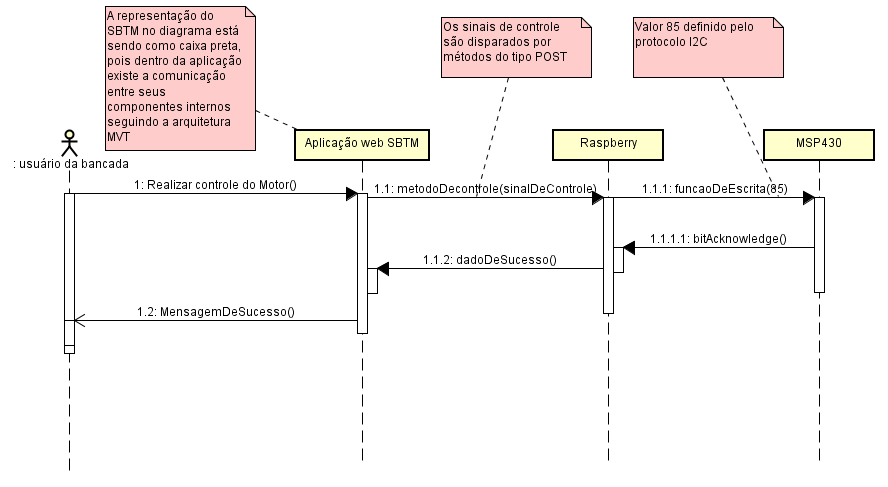
\includegraphics[keepaspectratio=true,scale= 0.7]{figuras/DiagramaDeSequenciaControle.PNG}
	\caption{Diagrama de sequência do modulo de controle}
	\label{diagramaControle}
\end{figure}

A Figura \ref{diagramaControle} acima representa todo o fluxo de processamento dos dados para o controle de acionamento e aceleração do motor, o detalhamento da aquisição é apresentado abaixo, desde a interação do usuário com a aplicação web até a chegada da requisição ao microcontrolador correspondente e vice e versa.

O passo a passo está descrito a seguir:

\begin{enumerate}
	\item O usuário acessa a aplicação SBTM através de um navegador Web:
		\begin{itemize}
			\item Caso o usuário corrente não possua cadastro, este deve cadastrar-se;
			\item Caso contrário, o usuário deverá autentica-se na aplicação.
		\end{itemize}
	\item O usuário é transferido para uma página onde poderá selecionar entre duas opções:
		\begin{itemize}
			\item Visualizar resultados de ensaios anteriores:
				\begin{itemize}
					\item A aplicação irá recuperar os dados referentes ao ensaio selecionado e os apresentará em forma de gráfico (Dados do sensores pelo Tempo) entre outras análises.
				\end{itemize}
			\item Iniciar um novo ensaio:
			\begin{itemize}
				\item A aplicação irá enviar uma mensagem de controle para o módulo de controle presente na Raspberry através de um \textit{Socket} TCP, que por sua vez envia um comando para a MSP de controle através do protocolo I$^{2}$C ordenando o acionamento do motor.
			\end{itemize}
		\end{itemize}
	\item A aplicação irá aguardar os primeiros dados de RPM do motor para iniciar a apresentação dos dados;
	
	\item Para o envio de dados dos sensores para a aplicação, A MSP enviará os dados por meio do protocolo I$^{2}$C para o módulo de aquisição da Raspberry que fará os cálculos de conversão dos dados de tensão para a unidade decimal e os transmitirá via \textit{Socket} UDP para a aplicação;
	
	\item A aplicação irá receber os dados oriundos dos sensores que serão tratados por duas \textit{threads}. Enquanto uma \textit{threads} ficará responsável pelo armazenamento das informações dos sensores no Banco de Dados da aplicação (Isso só ocorrerá um minuto após do ensaio ter sido iniciado) , a outra apresentará os dados na interface para o usuário no mesmo tempo em que são recebidos;
	
	\item Para determinar o término do ensaio a aplicação verificará se os dados de RPM ainda estão sendo transmitidos. Caso não, a aplicação encerrará o ensaio e o armazenamento das informações no Banco de Dados.
	
	\item 	Após o término do ensaio o usuário poderá ver os resultados do mesmo e adicionar uma descrição referente ao ensaio encerrado que será armazenada no Banco de Dados para uma visualização posterior.
\end{enumerate}


\section{Protocolos - Aquisição e Controle}

Para o módulo de controle, o protocolo de comunicação entre a aplicação web e a Raspberry Pi será via socket TCP, tendo em vista que este protocolo nos garante que a mensagem chegou ao seu destino que no caso será a Raspberry Pi. Assim, ao solicitar o envio de uma mensagem de controle pela aplicação (ligar o motor, por exemplo), um \textit{socket} é aberto para estabelecer uma conexão para o envio. A aplicação espera uma resposta por parte da Raspberry Pi indicando que a mensagem chegou com sucesso, e caso esta mensagem de retorno não chegue no tempo determinado (\textit{Timeout}) a aplicação envia a mensagem novamente.


Já para o módulo de aquisição, os dados dos sensores acoplados ao motor serão coletados por uma placa MSP-430 e transmitidos via protocolo I$^{2}$C para a Raspberry Pi que servirá como intermediadora entre a MSP-430 e a aplicação. O protocolo utilizado para a transmissão dos dados entre a Raspberry Pi e a aplicação web será o UDP. Tendo em vista o grande volume de dados a serem transmitidos, a justificativa da escolha deste protocolo é a sua alta taxa de transferência. Entretanto, o protocolo UDP não garante a chegada dos dados ao seu destino, porém, como o 
